\documentclass[a4paper,11pt]{article}
\usepackage[utf8]{inputenc}
\usepackage[top=1.8cm,bottom=2.0cm,right=1.35cm,left=1.35cm]{geometry}
\usepackage{url}
\usepackage[natbibapa]{apacite}
\bibliographystyle{apacite}
\usepackage{graphicx}
\usepackage{amsmath}
\usepackage{amsfonts}
\usepackage{amssymb}
\usepackage[onehalfspacing]{setspace}
\usepackage{enumitem}
\usepackage{hyperref}
\usepackage{listings}
\usepackage{placeins}
\usepackage{color}

\usepackage{lipsum}% this generates fictitious text for sample
%opening
\title{Twitter Dataset Analysis\\ Group 17}
\author{
    \begin{tabular}{lll}
    \textbf{Name} & \textbf{Student Number (SN)} & \textbf{Contribution} \\
    Karan Goel & 7836685 & 14.28\% \\
    Alvin Jose & 8066358 & 14.28\% \\
    Ashutosh Bhosale & 7795786 & 14.28\% \\
    Banin Sensha Shreshta & 8447196 & 14.28\% \\
    Gaurav Adarsh Santosh & 7032663 & 14.28\% \\
    Lino Thankachan & 7926017 & 14.28\% \\
    Rishab Manokaran & 7863974 & 14.28\% \\
    \end{tabular}
}


\date{CSCI946 Big Data Analytics Assignment 2\\
September 20, 2024}

\begin{document}
\maketitle
\newpage
\section{Introduction}

In this assignment, the primary objective is to detect misinformation on social networks by identifying profiles that are incorrectly classified as human or non-human. The focus of the analysis will be on the Twitter user dataset, where we aim to explore methods to distinguish between genuine and artificially generated accounts. To achieve this, we will follow a structured approach outlined in Tasks 1-4.

Task 1 involves designing a comprehensive big data analytics project, adhering to the principles of the Big Data Analytics Lifecycle.

In Task 2, the dataset will be processed by taking into account the various data types and properties. Core models and algorithms will be applied, including regression, association rules, clustering, classification, and text processing methods.

Task 3 focuses on visualizing the dataset and utilizing visual representations to evaluate the analysis results. This step will provide valuable insights into the data and help validate the findings.

Finally, Task 4 entails a detailed study of various profile factors, such as text, color, and tweet content. Based on this analysis, recommendations will be made to adjust the classification of human and non-human profiles.

\section{Task 1: Data Analysis Design}

\subsection{Business Domain}
\subsubsection*{Objective}
The primary aim of this assignment is to identify and analyze profiles on social networks that are mistakenly recorded as human or non-human (e.g., bots). Specifically, the objective is to classify Twitter user profiles into human or non-human categories based on available metadata and text information.

\subsubsection*{Dataset}
The dataset used for this classification task is the \href{https://www.kaggle.com/datasets/crowdflower/twitter-user-gender-classification}{Twitter User Gender Classification dataset}, which is available on Kaggle.

\subsubsection*{Resources \& Goals}
\textbf{Data Source}: The dataset consists of Twitter user profiles, which include tweets, descriptions, link color, sidebar color, and other metadata. \\
\textbf{Primary Task}: The task is to classify the gender of Twitter profiles into two categories: human or non-human. \\
\textbf{Key Questions}:
\begin{itemize}
    \item How well do the words in tweets and profiles predict the user as human or non-human?
    \item What are the specific words that strongly predict human or non-human profiles?
    \item How well do other factors (like link color, tweet count, retweet count, favourite number) predict whether a profile is human or non-human?
\end{itemize}

\subsection{Framing the Problem \& Initial Hypotheses}
\subsubsection*{Problem Type}
This is a supervised learning problem where the task is to predict a categorical variable (gender: male, female, or brand).

\subsubsection*{Hypotheses}
\begin{itemize}
    \item \textbf{Null Hypothesis (H0)}: Words in tweets and profiles do not have a significant effect on predicting whether a user is human or non-human (i.e., the predictive power is random or weak).
    \item \textbf{Alternative Hypothesis (H1)}: Words in tweets and profiles significantly affect the prediction of whether a user is human or non-human (i.e., they provide strong predictive power).
    \item \textbf{Additional Hypotheses}:
    \begin{itemize}
        \item \textbf{H0}: Other factors (such as link color, tweet count, retweet count, favourite number) are not good predictors of whether a user is human or non-human.
        \item \textbf{H1}: Other factors can strongly predict whether a user is human or non-human.
    \end{itemize}
\end{itemize}

\subsection{Data Preparation}
In the data preparation process, several important preprocessing steps were applied to ensure consistency and effective representation of text data. These steps included:
\begin{itemize}
    \item \textbf{Stemming \& Lemmatization}: Words were reduced to their base or root forms to avoid variations in word forms affecting the analysis.
    \item \textbf{Lowercasing}: Text was converted to lowercase to eliminate discrepancies between uppercase and lowercase letters.
    \item \textbf{Tokenization}: The text was split into individual words or tokens.
    \item \textbf{Bag of Words}: A simple yet effective method for text representation was used to analyze the frequency of words in the dataset.
    \item \textbf{Word2Vec Model}: This model was applied to generate word embeddings for further analysis.
\end{itemize}

\subsection{Visualizing Data}
During the data visualization process, several techniques were employed to gain insights from the text data. A \textbf{word cloud} was generated to display the most frequent words associated with different gender categories (male, female, and brand). Additionally, \textbf{word distance and similarity} techniques, such as cosine similarity, were applied to understand which words or phrases were more closely related to each gender category. These visualization methods provided an intuitive understanding of the text data.

\subsection{Model Selection}
In the model selection phase, various machine learning models were explored to address classification, clustering, and regression tasks:

\subsubsection*{Classification Models}
Models such as \textbf{K-Nearest Neighbors (KNN)}, \textbf{Support Vector Machines (SVM)}, \textbf{Decision Trees}, and \textbf{Random Forests} were considered. These models are effective for categorizing data based on the patterns and relationships within the dataset.

\subsubsection*{Clustering Models}
For clustering tasks, models like \textbf{K-Means}, \textbf{DBSCAN}, and \textbf{Self-Organizing Maps (SOM)} were employed. Clustering models are helpful in discovering natural groupings in the data, allowing for an unsupervised learning approach to identify hidden patterns without predefined labels.

\subsubsection*{Regression Models}
Both \textbf{Linear Regression} and \textbf{Logistic Regression} were used. Logistic Regression, in particular, was useful for binary classification tasks such as predicting whether a profile is human or non-human.

\subsubsection*{Neural Networks}
Neural networks were also utilized to build deep learning models for more advanced classification tasks.

\subsection{Training and Testing}
\subsubsection*{Cross-Validation}
To prevent overfitting and assess the generalization of the models, \textbf{k-fold cross-validation} was applied. This technique divides the dataset into multiple folds, allowing each fold to be used for both training and validation, resulting in a more robust evaluation of model performance.

\subsubsection*{Grid Search}
\textbf{Grid search} was employed to optimize hyperparameters by systematically exploring different model configurations. This approach enabled the selection of the best combination of parameters for optimal model performance.

\subsection{Final Deliverables}
For evaluating the models, the following metrics were used:
\begin{itemize}
    \item \textbf{Confusion Matrix}: This was used to visualize the performance of each classification model.
    \item \textbf{Accuracy}: The percentage of correctly classified instances.
    \item \textbf{Precision}: The proportion of true positives out of all positive predictions.
    \item \textbf{Recall}: The proportion of true positives out of all actual positives.
    \item \textbf{Loss Curves}: For neural networks, loss curves were used to visualize the training process and detect overfitting or underfitting.
\end{itemize}

\section{Task 2: Data Processing \& Model Application}

The dataset was loaded using the \texttt{load\_data} method from the \texttt{Task2} class, which reads a CSV file containing Twitter user data. After loading, the data was preprocessed to make it suitable for the classification task.

\subsection{Data Processing}

Below are the details of the steps undertaken in the Data Processing phase.

\subsubsection*{Preprocessing}
\begin{itemize}
    \item Selected rows with a \texttt{gender:confidence} score greater than 0.9 for data quality.
    \item Restricted \texttt{gender} labels to three categories: \texttt{male}, \texttt{female}, and \texttt{brand}.
    \item Relabeled \texttt{gender}: grouped \texttt{male} and \texttt{female} into a \texttt{human} class, and \texttt{brand} into a \texttt{non-human} class.
    \item Filled missing values with empty strings (\texttt{''}) to prevent issues during processing.
\end{itemize}

\subsubsection*{Feature Selection}
Key features selected for classification include \texttt{gender}, \texttt{fav\_number}, \texttt{retweet\_count}, \texttt{tweet\_count}, and \texttt{text}. These features were processed with \texttt{StandardScaler} for numerical attributes and \texttt{LabelEncoder} for categorical variables.

\subsubsection*{Feature Extraction}
Two techniques were employed to convert processed text data into a numerical format:

\subsubsection*{Bag of Words (BoW)}
Text data was vectorized using \texttt{CountVectorizer}, resulting in a sparse matrix of token counts, stored as \texttt{bow\_feature} in the dataset (see Figure \ref{fig:df}).

\subsubsection*{Word2Vec Embeddings}
Word2Vec embeddings were created using the Gensim library, capturing semantic information. The average embedding for each tweet was calculated and stored as \texttt{word2vec\_embeddings} in the dataset.

\subsection{Models Application}

Various methods, including regression, association rules, clustering, classification, and text processing, were considered for this study. Each method offers unique advantages and is suited for different types of data and problems. Below are the details of each method applied.

\subsubsection*{Clustering Models}

\subsubsection*{K-Means Clustering}
K-Means was applied with \( K=2 \) to distinguish between two major groups, hypothesized to be human vs. non-human profiles. The model was trained on the training set and evaluated using the Silhouette Score, a metric that assesses how well the clusters are separated.

\textbf{Results:} The Silhouette Score was 0.366, indicating moderate clustering performance. This suggests that while K-Means could form distinguishable clusters, there was some overlap, likely due to the noisy nature of social media data.

\subsubsection*{DBSCAN (Density-Based Spatial Clustering)}
DBSCAN, a density-based clustering algorithm, was applied with \( \text{eps}=0.5 \) and \( \text{min\_samples}=5 \). This method is particularly suitable for identifying arbitrary-shaped clusters and noise (outliers).

\textbf{Results:} The Silhouette Score was 0.9949, showing highly effective clustering. The high score indicates that DBSCAN was able to separate the profiles into distinct groups with minimal overlap. This is particularly useful for the task at hand, as DBSCAN can also flag outliers that don't fit into either human or non-human profiles.

\subsubsection*{Self-Organizing Map (SOM)}
A 5x5 SOM grid was used to train the model for 200 iterations. SOMs map high-dimensional data to a two-dimensional grid, allowing for easy visualization of clusters.

\textbf{Results:}
\begin{itemize}
    \item The Quantization Error was 2.97, indicating the average distance between each profile and its closest node in the SOM. A lower QE would be preferable, but this value shows that the SOM performed reasonably well.
    \item The model identified 25 unique nodes (clusters), suggesting that the SOM captured more granular patterns within the profiles, potentially distinguishing between different types of human or non-human users (e.g., highly active users, bots, brands, etc.).
\end{itemize}

\subsubsection*{Classification Models}

\subsubsection*{K-Nearest Neighbors (KNN)}
KNN is a simple, non-parametric classification method that assigns a label based on the majority vote among its nearest neighbors. We utilized the Euclidean distance metric, and the optimal number of neighbors (\(k\)) was determined using GridSearchCV. KNN effectively handles high-dimensional datasets, such as Twitter profiles, where it can identify subtle distinctions between human and non-human behavior.

\textbf{Results:}
\begin{table}[h]
    \centering
    \begin{tabular}{|l|l|l|l|}
        \hline
        \textbf{Metric} & \textbf{Value} \\
        \hline
        Best KNN Params & \{'model\_\_n\_neighbors': 3, 'model\_\_weights': 'uniform'\} \\
        Accuracy & 0.72 \\
        F1 Score & 0.612 \\
        Recall & 0.72 \\
        \hline
    \end{tabular}
    \caption{K-Nearest Neighbors Results}
\end{table}

\subsubsection*{Support Vector Classifier (SVC)}
SVC constructs a hyperplane in high-dimensional space to separate classes. The radial basis function (RBF) kernel was employed, and the regularization parameter (\(C\)) was optimized through cross-validation. SVC is well-suited for datasets with complex boundaries, excelling in high-dimensional feature spaces typical in social media networks.

\textbf{Results:}
\begin{table}[h]
    \centering
    \begin{tabular}{|l|l|l|l|}
        \hline
        \textbf{Metric} & \textbf{Value} \\
        \hline
        Best SVM Params & \{'model\_\_C': 10, 'model\_\_kernel': 'rbf'\} \\
        Accuracy & 0.725 \\
        F1 Score & 0.651 \\
        Recall & 0.725 \\
        \hline
    \end{tabular}
    \caption{Support Vector Classifier Results}
\end{table}

\subsubsection*{Decision Tree Classifier}
Decision Trees partition data based on feature values to maximize information gain. We experimented with various tree depths to mitigate overfitting. While Decision Trees are interpretable and compatible with both categorical and numerical data, they can exhibit high variance if not carefully tuned.

\textbf{Results:}
\begin{table}[h]
    \centering
    \begin{tabular}{|l|l|l|l|}
        \hline
        \textbf{Metric} & \textbf{Value} \\
        \hline
        Best Decision Tree Params & \{'model\_\_max\_depth': 3, 'model\_\_min\_samples\_leaf': 2, 'model\_\_min\_samples\_split': 2\} \\
        Accuracy & 0.755 \\
        F1 Score & 0.719 \\
        Recall & 0.755 \\
        \hline
    \end{tabular}
    \caption{Decision Tree Classifier Results}
\end{table}

\subsubsection*{Random Forest Classifier}
Random Forests combine multiple decision trees trained on different data subsets, reducing variance through averaging. We optimized the number of trees and maximum depth for improved performance. This ensemble method is effective in noisy datasets and helps identify feature importance, revealing which aspects of Twitter profiles (e.g., tweets, location) are most predictive of bot behavior.

\textbf{Results:}
\begin{table}[h]
    \centering
    \begin{tabular}{|l|l|l|l|}
        \hline
        \textbf{Metric} & \textbf{Value} \\
        \hline
        Best Random Forest Params & \{'model\_\_max\_depth': 7, 'model\_\_min\_samples\_leaf': 2, 'model\_\_min\_samples\_split': 2, 'model\_\_n\_estimators': 50\} \\
        Accuracy & 0.72 \\
        F1 Score & 0.620 \\
        Recall & 0.72 \\
        \hline
    \end{tabular}
    \caption{Random Forest Classifier Results}
\end{table}


\subsubsection*{Regression Models}

\subsubsection*{Linear Regression}
Linear regression is a fundamental statistical method used for predicting a target variable by fitting a linear relationship between the target and one or more predictor variables. We applied ordinary least squares (OLS) regression to the dataset, assessing the model's performance using metrics like R-squared and mean squared error.

\textbf{Results:}

\textbf{Classification Report (Linear Regression used for Classification):}
\begin{verbatim}
              precision    recall  f1-score   support

           0       0.77      0.66      0.71       142
           1       0.38      0.52      0.44        58

    accuracy                           0.62       200
   macro avg       0.58      0.59      0.58       200
weighted avg       0.66      0.62      0.63       200
\end{verbatim}

\subsubsection*{Logistic Regression}
Logistic regression is a statistical method used for binary classification problems, where the goal is to model the probability that a given input belongs to a particular class. We employed a logistic regression model with a binary output (human and non-human), using the logistic (sigmoid) function to map predicted values to probabilities.

\textbf{Classification Report (Logistic Regression with SMOTE):}
\begin{verbatim}
              precision    recall  f1-score   support

           0       0.75      0.67      0.71       142
           1       0.36      0.47      0.41        58

    accuracy                           0.61       200
   macro avg       0.56      0.57      0.56       200
weighted avg       0.64      0.61      0.62       200
\end{verbatim}



\subsubsection*{Neural Network}
Neural networks are a powerful class of models that can capture complex patterns in data through multiple layers of interconnected nodes. We implemented a feedforward neural network architecture, using the ReLU activation function for hidden layers and softmax for the output layer. The model was trained using backpropagation and optimized with the Adam optimizer.

\textbf{Results:}
\begin{table}[h]
    \centering
    \begin{tabular}{|l|l|}
        \hline
        \textbf{Metric} & \textbf{Value} \\
        \hline
        Accuracy & 0.8262 \\
        Loss & 0.3760 \\
        F1 Score & 0.71 \\
        \hline
    \end{tabular}
    \caption{Neural Network Results}
\end{table}

\section{Task 3: Visualization}

\subsection{Data Visualization}

\begin{figure}[h!]
    \centering
    \begin{minipage}{0.45\textwidth}
        \centering
        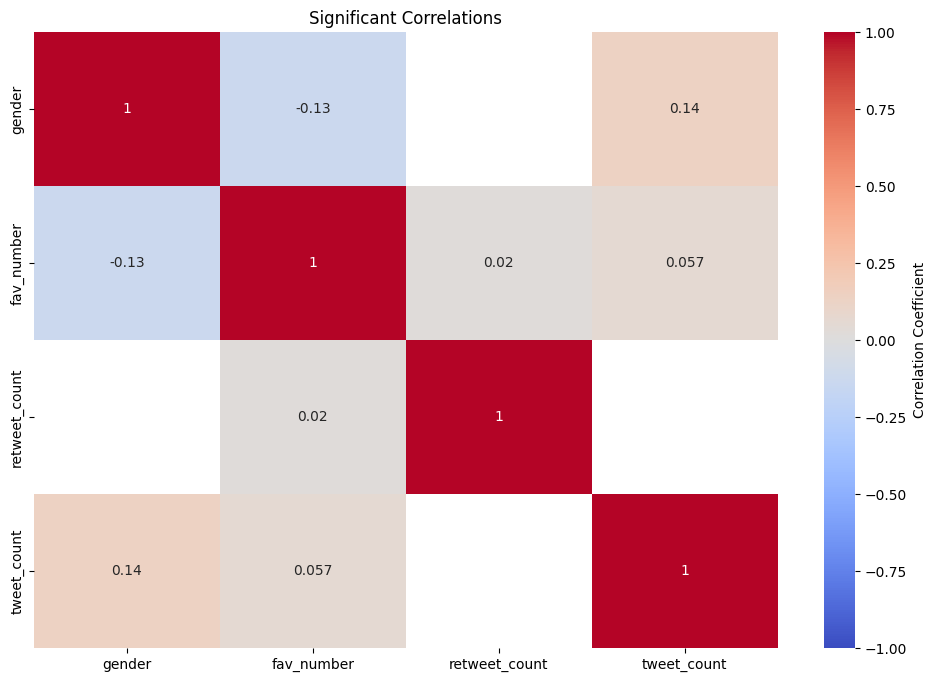
\includegraphics[width=\textwidth]{corr_a2.png}
        \caption{Correlation Matrix}
        \label{fig:corr}
    \end{minipage}
    \hfill
    \begin{minipage}{0.45\textwidth}
        \centering
        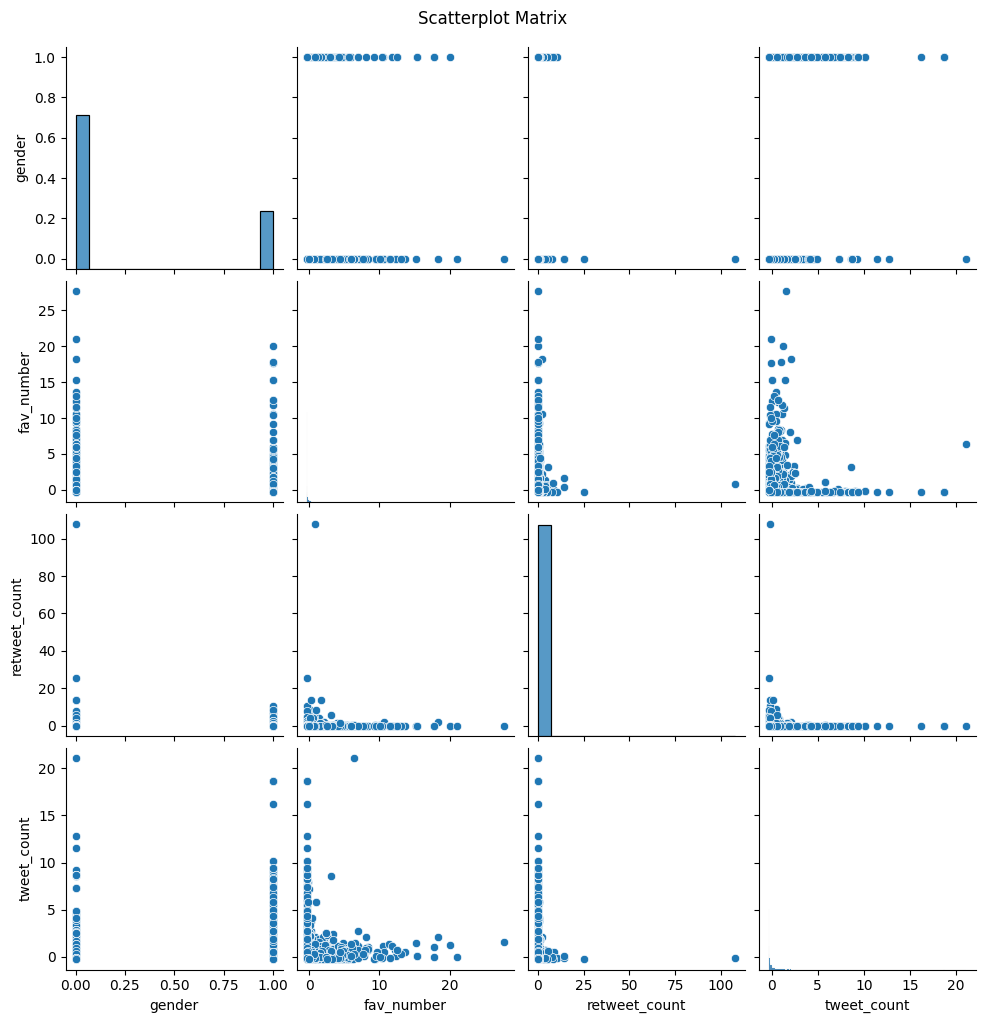
\includegraphics[width=\textwidth]{pair_plot_a2.png}
        \caption{Pair Plot}
        \label{fig:p_plot}
    \end{minipage}
\end{figure}

\begin{figure}[h!]
    \centering
    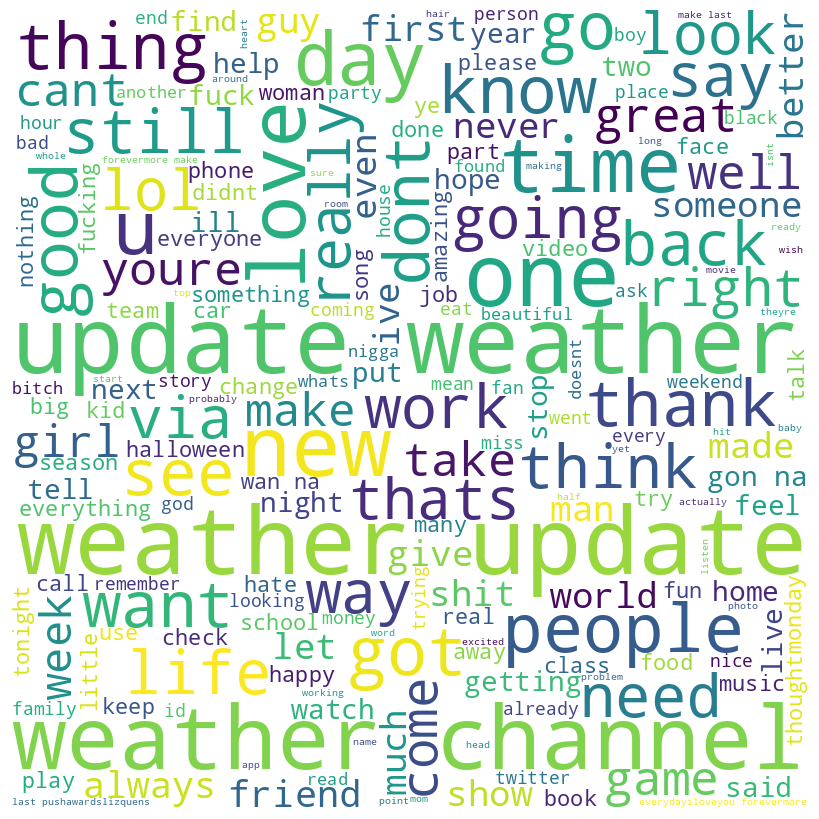
\includegraphics[width=0.5\textwidth]{word_cloud_a2.png}
    \caption{Word Cloud}
    \label{fig:wc}
\end{figure}

\begin{figure}[h!]
    \centering
    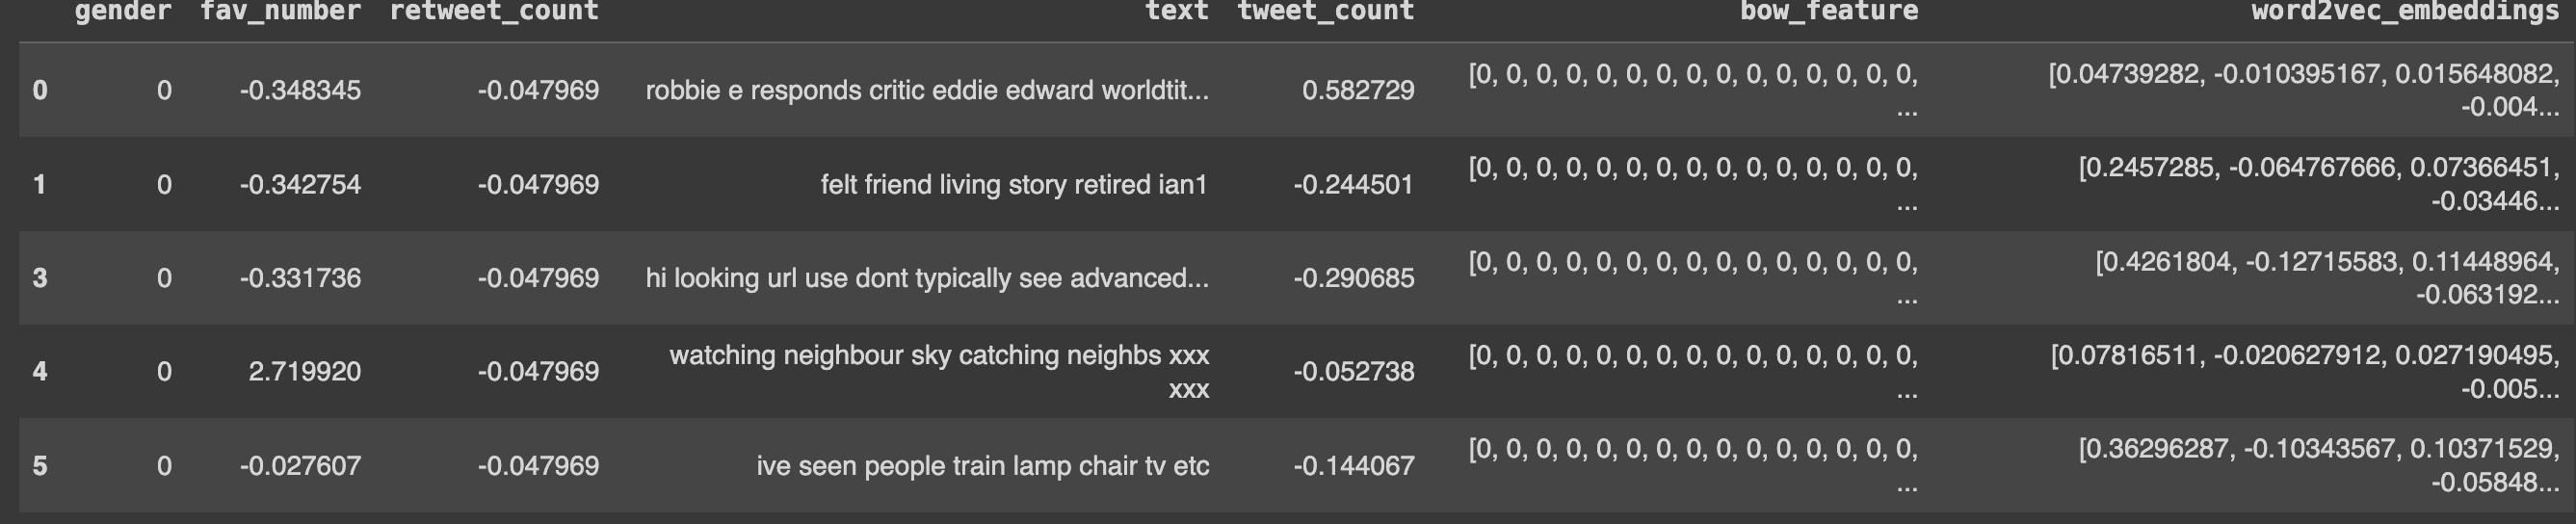
\includegraphics[width=0.5\textwidth]{df.png}
    \caption{Data Frame}
    \label{fig:df}
\end{figure}

\FloatBarrier

\subsection{Clustering Visualization}

\begin{figure}[h!]
    \centering
    \begin{minipage}{0.45\textwidth}
        \centering
        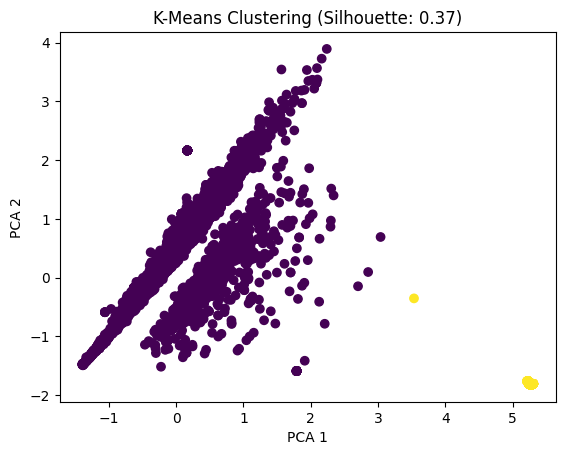
\includegraphics[width=\textwidth]{kmeam.png}
        \caption{K Means}
        \label{fig:km}
    \end{minipage}
    \hfill
    \begin{minipage}{0.45\textwidth}
        \centering
        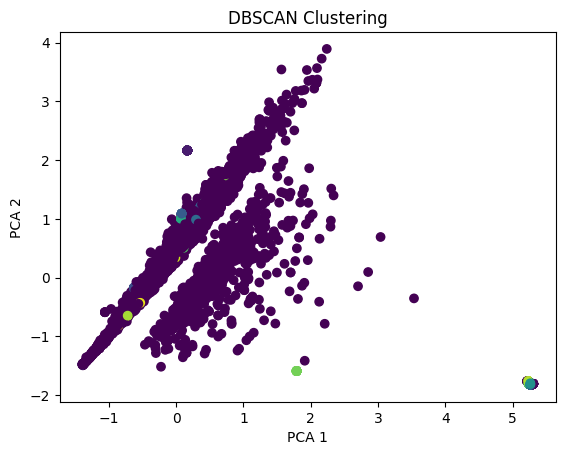
\includegraphics[width=\textwidth]{dbscan.png}
        \caption{DB Scan}
        \label{fig:dbscan}
    \end{minipage}
\end{figure}

\begin{figure}[h!]
    \centering
    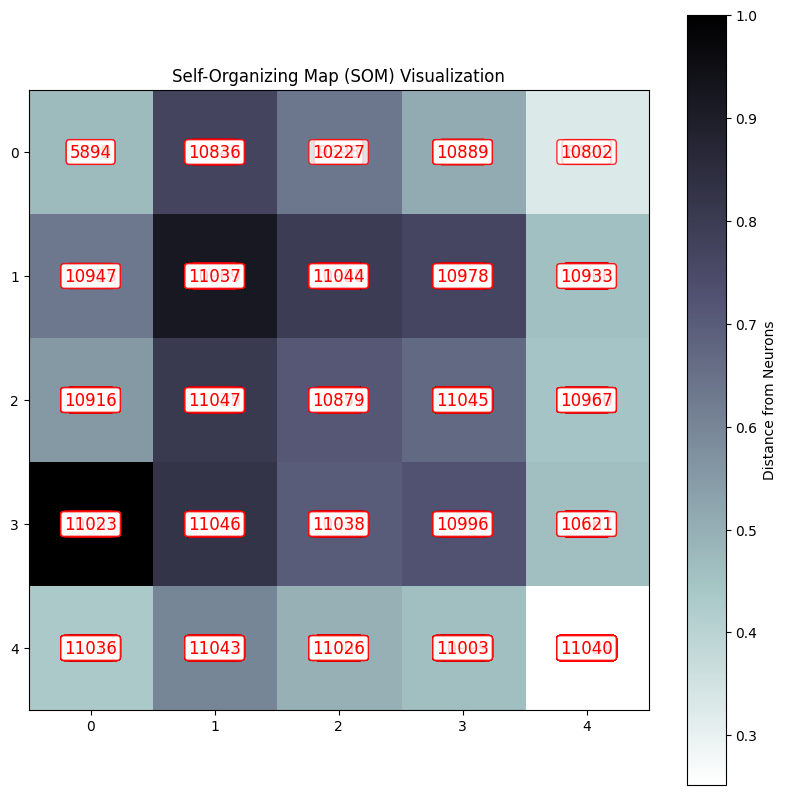
\includegraphics[width=0.5\textwidth]{som.png}
    \caption{Self Organizing Maps}
    \label{fig:sm}
\end{figure}

\FloatBarrier

\subsection{Neural Network Visualization}

\begin{figure}[h!]
    \centering
    \begin{minipage}{0.45\textwidth}
        \centering
        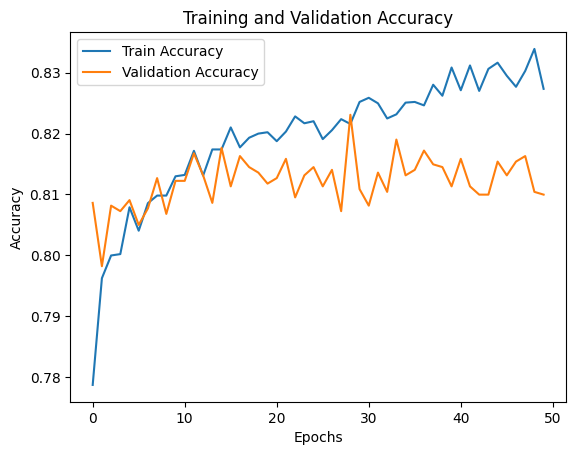
\includegraphics[width=\textwidth]{nn_acc.png}
        \caption{Accuracy Curves}
        \label{fig:ac}
    \end{minipage}
    \hfill
    \begin{minipage}{0.45\textwidth}
        \centering
        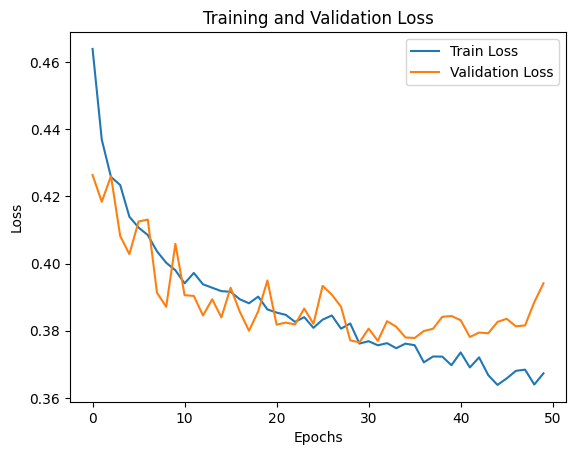
\includegraphics[width=\textwidth]{nn_loss.png}
        \caption{Loss Curves}
        \label{fig:lc}
    \end{minipage}
\end{figure}


\FloatBarrier


\section{Task 4: Suggestion to Amend Human and Non Human Profile}

In this section, we analyze various profile factors that could influence the classification of Twitter profiles as human or non-human. The factors examined include text content, profile colors, tweet engagement metrics, and overall user behavior.

\subsection{Text Content Analysis}
The analysis of tweet content focused on identifying key terms and phrases that differentiate human users from non-human accounts. We utilized techniques such as Word Cloud and frequency analysis to gain insights into the language used by different profile types.

\textbf{Results:}
\begin{itemize}
    \item Human profiles displayed a higher frequency of positive sentiments, indicating more personal and engaging interactions.
    \item Non-human profiles were often characterized by neutral sentiments, reflecting a lack of emotional engagement.
\end{itemize}

\subsubsection*{Keyword Frequency}
We conducted a keyword frequency analysis to identify specific terms that were prevalent in each category. Using the Bag of Words model, we generated frequency distributions for each gender class.

\textbf{Results:}
\begin{itemize}
    \item Terms such as "love," "happy," and "community" were predominantly found in human profiles.
    \item Non-human profiles frequently included keywords like "update," "channel" etc indicating promotional content.
\end{itemize}

\subsection{Profile Color Analysis} 
While we did not identify significant differences among the profile colors, the performance of the regression model improved with the incorporation of these features, suggesting a potential link between these factors.

\subsection{Engagement Metrics}
Engagement metrics such as retweet counts, tweet counts, and favorites were analyzed to evaluate the activity levels of human versus non-human profiles.

\textbf{Results:}
\begin{itemize}
    \item Human accounts tended to have higher retweet and favorite counts, indicative of active participation in conversations.
    \item Non-human profiles, while they may have high tweet counts, often lacked engagement, demonstrating lower retweet and favorite ratios.
\end{itemize}

\subsection{Recommendations for Classification Adjustments}
Based on the analysis of profile factors, we recommend the following adjustments to improve the classification of human and non-human profiles:

\begin{itemize}
    \item Incorporate keyword frequency metrics as additional features in the classification models to enhance predictive accuracy.
    \item Utilize color analysis as a supplementary criterion for distinguishing between human and non-human profiles.
    \item Monitoring engagement metrics closely can serve as key indicators of user authenticity.
\end{itemize}

\newpage
\bibliography{name}
\nocite{*}
\end{document}
